\documentclass[12pt,letterpaper]{paper}
\usepackage[utf8]{inputenc}
\usepackage{amsmath}
\usepackage{amsfonts}
\usepackage{amssymb}
\usepackage[left=.5in, right=.25in, top=1.00in, bottom=1.00in]{geometry}
%\usepackage[left=1.00cm, right=1.00cm, top=1.00cm, bottom=1.00cm]{geometry}
\usepackage[pdftex]{graphicx} 
%opening
\title{COSMOS Orbit and Attitude Propagation Algorithms}
\author{Eric J. Pilger, Miguel A. Nunes}

\begin{document}

\maketitle
\noindent
Last Revision: \today
\tableofcontents

\section{Terms and Usage}
The COSMOS environment supports propagation of both a Position and Attitude state for objects. 
\subsection{Units}
All units, unless otherwise indicated, are SI, with angles expressed in radians. All absolute times (eg. dates) are expressed in Modified Julian Days (MJD).
\subsection{Time}
Important time scales
\begin{itemize}
\item TAI, International Atomic Time: in units of SI seconds
\item UTC, Coordinated Universal Time: basis of civil time, in units of SI seconds, but jumps periodically to keep within 0.9 seconds of UT1.
\item UT1, Universal Time: Human time scale, tied to the irregular rotation of the earth, measured at 0 degrees longitude.
\item ERA, Earth Rotation Angle: with respect to ICRF
\item EEQ, Equation of the Equinoxes
\item GAST, ERA + EEQ
\item TT, Terrestrial Time: used with ephemerides, in units of SI seconds, ahead of TAI by 32.184 seconds.
\item GPS, GPS Time: used with GPS, in units of SI seconds, behind TAI by 19. seconds.
\end{itemize}
Important representations.
\begin{itemize}
\item Julian Day (JD) - number of days since 12:00 UT on January 1, 4713 BC
\item Modified Julian Day (MJD) - number of days since 00:00 UT, November 17, 1858
\end{itemize}
\subsection{Rotations and Transformations}
Vector rotations represent the physical motion of a vector within a single coordinate system. Vector transformations represent the conversion of the coordinates of a vector in one coordinate system into the coordinates of the same vector in a second coordinate system (or the rotation of the axes of the first coordinate system into the axes of the second). The quaternion representation chosen is that which produces rotation with a Left Side Multiplication.
\section{Time Calculation}
UTC is used as the base time for all operations. It is converted to and from all other time frames as needed using the equations below.
\subsection{Equations}
\begin{equation}
UT1 = UTC + {\Delta}UT1
\end{equation}
where ${\Delta}UT1$ is provided by IERS bulletins A and B, and expressed in days.
\begin{equation}
TT = UTC + (32.184 + LS)/86400.
\end{equation}
where LS is the number of leap seconds as provided by IERS bulletins B and C.
\begin{equation}
GPS = UTC - 51.184/86400.
\end{equation}
\begin{equation}
MJD = JD - 2400000.5
\end{equation}

\section{Orbital Position Propagation}
The full Position state is expressed as a Time, a Position(0th time derivative) ${r}_{ijk}$, a Rate(1st time derivative) ${v}_{ijk}$, and an Acceleration(2nd time derivative) ${a}_{ijk}$. Time is UTC stored as Modified Julian Day. COSMOS supports a variety of position source frames, and provides functions to synchronize all the frames for a complete Position and Attitude state from a specified updated frame. The currently supported position frames include:
\begin{itemize}
\item ICRF - aligned with the axes of the International Celestial Reference System, origin is at the barycenter of the solar system.
\item GCRF, Geocentric Celestial Reference Frame. Similarly to the ICRF this is an inertial frame, but centered at the Earth (geocentric). This is the standard inertial coordinate system for the Earth. Sometimes refered to as ECI. Aligned with the axes of the International Celestial Reference System.
\item J2000 - IAU-76/FK5 frame, differing from GCRF by a frame bias.
\item MOD - Mean of Date, differing from J2000 due to the Proper Motion of the Earth around the Sun.
\item TOD - True of Date, differing from MOD due to the Nutation of the Earth's axes.
\item PEF - Pseudo Earth Fixed, differing from TOD due to a rotation around Z-axis of GAST
\item ITRF, International Terrestrial Reference Frame. The ITRF is a realization of the International Terrestrial Reference System (ITRS). This is a Earth fixed (geocentric) coordinate system. The origin of this frame is at the center of the Earth. It is sometimes referred to as the Earth Centered, Earth Fixed (ECEF) frame.
\item SELC - aligned with axes of the Moon for the given time
\end{itemize}


%-------------------------------------------------
\subsection{Reductions}
The transformation from celestial to terrestrial coordinates in COSMOS is done using the IAU-76/FK5 reduction. This formulation is properly described in various sources such as in \cite{Vallado2013,Luzum2010,Vallado2006,Seago2000,Vallado2006a,Capitaine2003,Pottasch1997}. In 2000 the IAU adopted the updated models for computing the Earth's instantaneous orientation within the ICRS (\cite{Luzum2010}, chapter 5). But the classical reduction of IAU-76/FK5 is still precise enough for current applications we have adopted it for the current version of COSMOS. This classical transformations 

\subsection{Two Line Elements (TLE) to GCRF (ECI) coordinates}

The orbit propagation from a Two Line Element (TLE) state is propagated by an SGP4 algorithm that outputs the results in a true equator, mean equinox (TEME) coordinate system. Then we take the state in TEME and convert it to GCRF coordinates using multiple steps as described in the following sections. In essence the transformation is expressed by the following rotation matrices:

\begin{equation}
%\begin{align}
\mathbf{r}_{GCRF} = P N R_3(-Eq_{equinox1982}) \mathbf{r}_{TEME}
%\end{align}
\end{equation}

where $N$ is the nutation matrix and $P$ is the precession matrix. These steps in can also be seen as the sequential rotation of different reference frames $TEME \rightarrow TOD \rightarrow MOD \rightarrow J2000 \rightarrow GCRF $

\subsubsection{TEME to TOD}
The first step is to convert TEME coordinates to true equator of date (TOD). This is achieved by rotating the TEME coordinates around the Z-axis by the angle given by the Equation of the Equinox $Eq_{equinox1982}$.
\begin{equation}
%\begin{align}
\mathbf{r}_{TOD} = R_3(-Eq_{equinox1982}) \mathbf{r}_{TEME}
%\end{align}
\end{equation}



\subsubsection{TOD to MOD}
The second step is to convert TOD coordinates to mean equator of date (MOD). This is achieved by rotating the TOD coordinates by the rotation matrix that represents the nutation of the planet $N$. 

\begin{equation}
%\begin{align}
\mathbf{r}_{MOD} = N \mathbf{r}_{TOD}
%\end{align}
\end{equation}

The nutation matrix is given by
\begin{equation}
N = R_1(- \bar{\epsilon}_{1980})R_3(\Delta\Psi_{1980})R_1(\epsilon_{1980})
\end{equation}
where $R_i$ is the rotation about axis-i that represents the accumulated nutation angles $\epsilon_{1980}, \Delta\Psi_{1980}, \epsilon_{1980}$. These angular quantities can be computed by the following equations:
\begin{align}
\epsilon_{1980} &= \bar{\epsilon}_{1980} + \Delta \epsilon_{1980} \\
\bar{\epsilon}_{1980} &= 84,381.448'' - 46.8150T_{TT} - 0.00059T^2_{TT} + 0.001813 T^3_{TT}
\end{align}

The other terms are computed by evaluating a trigonometric series to find the nutation in longitude, $\Delta\Psi_{1980}$ and the nutation in obliquity,  $\Delta \epsilon_{1980}$

\begin{align}
\Delta \epsilon_{1980} &= \sum_{i=1}^{106} (C_i + D_i T_{TT})cos\left\lbrace{a_{p_i}}\right\rbrace \\
\Delta \Psi_{1980} &= \sum_{i=1}^{106} (A_i + B_i T_{TT})sin\left\lbrace{a_{p_i}}\right\rbrace
\end{align}



\subsubsection{MOD to J2000}
The third step is to convert MOD to J2000. This is done by rotating the MOD coordinates by the rotation matrix that represents precession of the planet:
\begin{equation}
P = R_3(-z)R_2(\theta)R_3(-\zeta)
\end{equation}
where $R_i$ is the rotation about axis-i that represents the accumulated precession angles $\zeta, \theta, z$ that specify the position of the mean equinox and equator of date w.r.t. the mean equinox and equator of standard epoch J2000.

%\begin{equation}
\begin{align}
\zeta &= 2306''.2181T + 0''.30188T^2 + 0''.0.17988T^3\\
\theta &= 2004''.3109T - 0''.42665T^2 - 0''.041833T^3\\
z &= 2306''.2181T + 1''.09468T^2 + 0''.018203T^3
\end{align}
%\end{equation}


\subsubsection{J2000 to GCRF}
Finally, we convert J2000 coordinates to GCRF coordinates by applying the following transformation

\begin{align}
\mathbf{r}_{GCRF} =  \begin{bmatrix}
        0.99999999999999 & -0.0000000707827974 & 0.0000000805621715 \\
        0.0000000707827948 & 0.9999999999999969 & 0.0000000330604145 \\
        -0.0000000805621738 & -0.0000000330604088 & 0.9999999999999962
     \end{bmatrix}^T \mathbf{r}_{J2000}
\end{align}


\subsection{Compare COSMOS results with STK}

In this section we validate the algorithms implemented in COSMOS by comparing the results with STK. we use an updated TLE file for the ISS to compare the results. Figures \ref{fig:compare_cosmos_stk_tle2gcrf_pos_error_x},\ref{fig:compare_cosmos_stk_tle2gcrf_pos_error_y},\ref{fig:compare_cosmos_stk_tle2gcrf_pos_error_z}\ref{fig:compare_cosmos_stk_tle2gcrf_pos_error_abs} show the comparison between the ISS position given STK data and a COSMOS test run for one week. The algorithm has a consistent error bounded between -2 and 2 meters for the difference in position in each of the three coordinates. Figures \ref{fig:compare_cosmos_stk_tle2gcrf_vel_error_x},\ref{fig:compare_cosmos_stk_tle2gcrf_vel_error_y},\ref{fig:compare_cosmos_stk_tle2gcrf_vel_error_z},\ref{fig:compare_cosmos_stk_tle2gcrf_vel_error_abs} show the error for the velocity. 

\begin{figure}
\centering
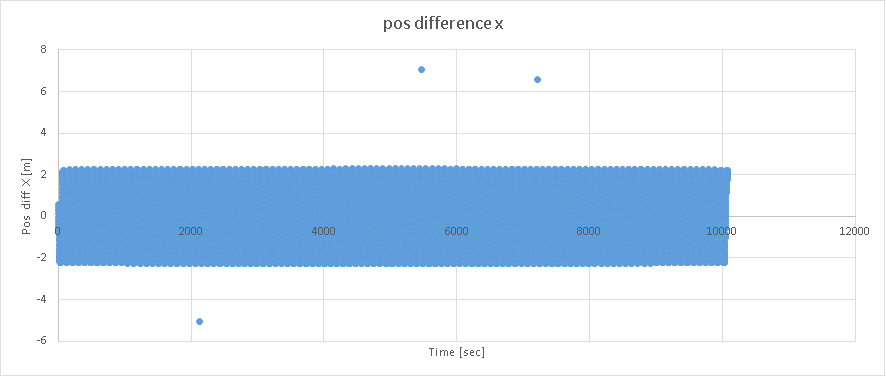
\includegraphics[width=0.9\linewidth]{figures/compare_cosmos_stk_tle2gcrf_pos_error_x}
\caption{X Position error in meters, difference between the results produced by the COSMOS algorithms and STK for one week run.}
\label{fig:compare_cosmos_stk_tle2gcrf_pos_error_x}
\end{figure}

\begin{figure}
\centering
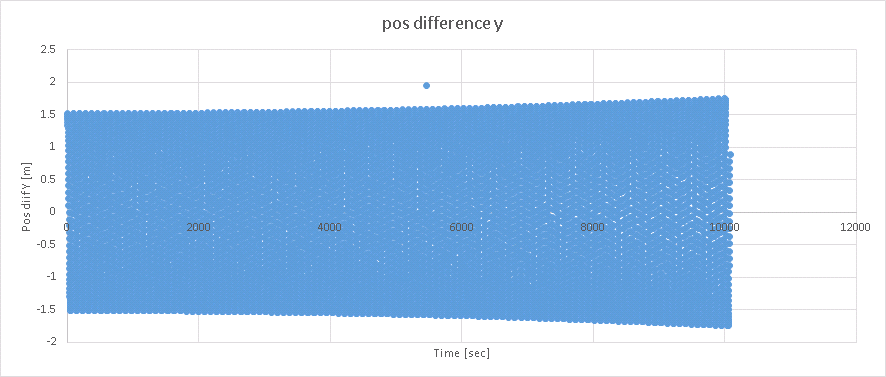
\includegraphics[width=0.9\linewidth]{figures/compare_cosmos_stk_tle2gcrf_pos_error_y}
\caption{Y Position error in meters, difference between the results produced by the COSMOS algorithms and STK for one week run}
\label{fig:compare_cosmos_stk_tle2gcrf_pos_error_y}
\end{figure}


\begin{figure}
\centering
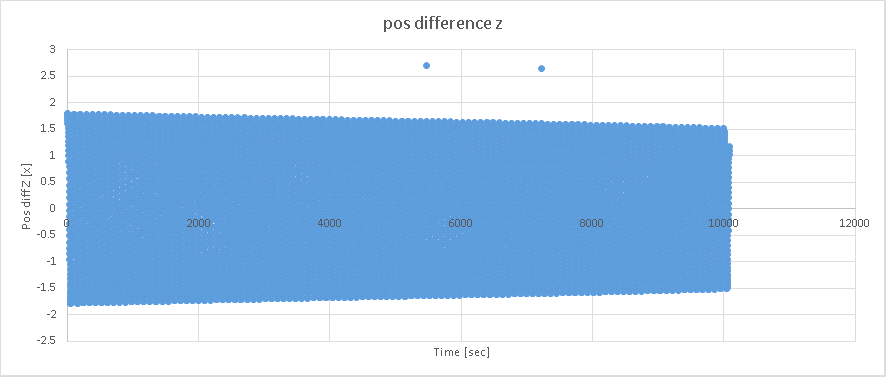
\includegraphics[width=0.9\linewidth]{figures/compare_cosmos_stk_tle2gcrf_pos_error_z}
\caption{Z Position error in meters, difference between the results produced by the COSMOS algorithms and STK for one week run}
\label{fig:compare_cosmos_stk_tle2gcrf_pos_error_z}
\end{figure}


\begin{figure}
\centering
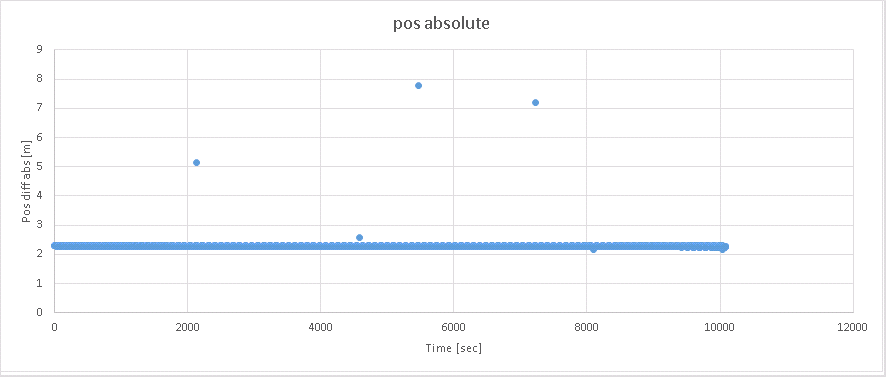
\includegraphics[width=0.9\linewidth]{figures/compare_cosmos_stk_tle2gcrf_pos_error_abs}
\caption{Absolute Position error in meters, difference between the results produced by the COSMOS algorithms and STK for one week run}
\label{fig:compare_cosmos_stk_tle2gcrf_pos_error_abs}
\end{figure}








\begin{figure}
\centering
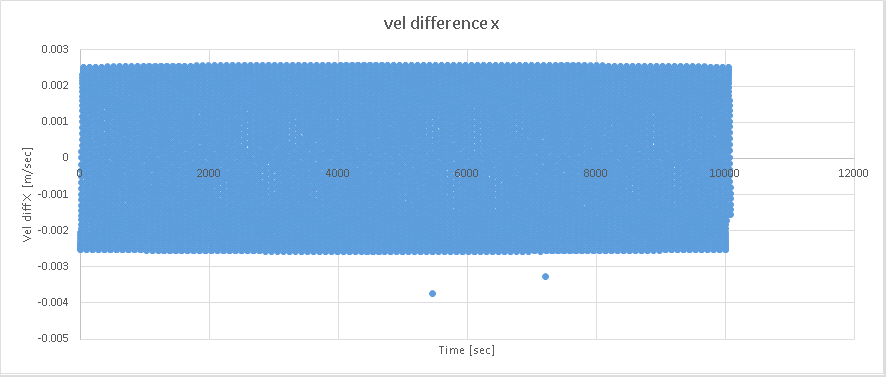
\includegraphics[width=0.9\linewidth]{figures/compare_cosmos_stk_tle2gcrf_vel_error_x}
\caption{X Velocity error in meters/sec, difference between the results produced by the COSMOS algorithms and STK for one week run}
\label{fig:compare_cosmos_stk_tle2gcrf_vel_error_x}
\end{figure}

\begin{figure}
\centering
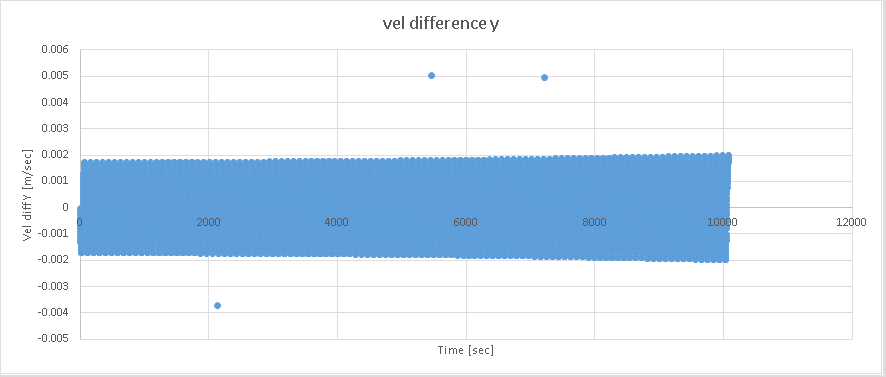
\includegraphics[width=0.9\linewidth]{figures/compare_cosmos_stk_tle2gcrf_vel_error_y}
\caption{Y Velocity error in meters/sec, difference between the results produced by the COSMOS algorithms and STK for one week run}
\label{fig:compare_cosmos_stk_tle2gcrf_vel_error_y}
\end{figure}


\begin{figure}
\centering
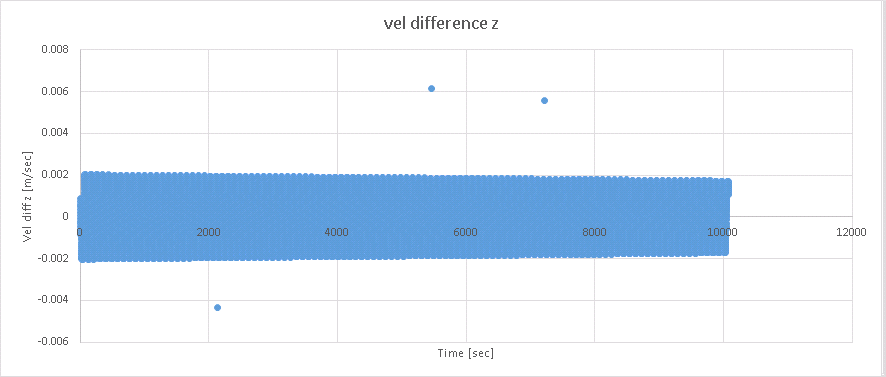
\includegraphics[width=0.9\linewidth]{figures/compare_cosmos_stk_tle2gcrf_vel_error_z}
\caption{Z Velocity error in meters/sec, difference between the results produced by the COSMOS algorithms and STK for one week run}
\label{fig:compare_cosmos_stk_tle2gcrf_vel_error_z}
\end{figure}


\begin{figure}
\centering
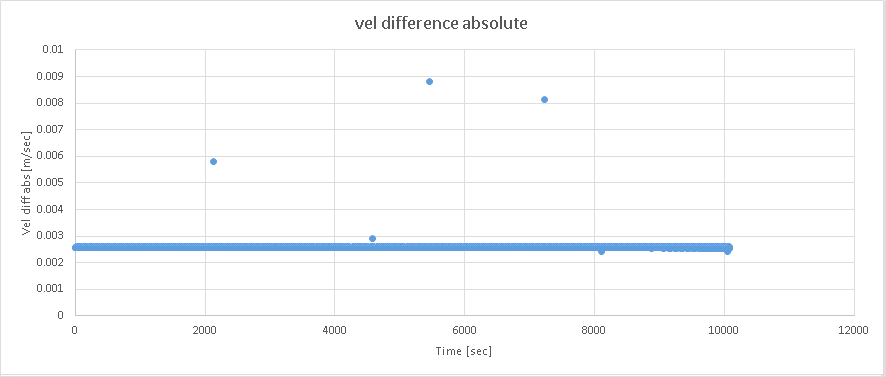
\includegraphics[width=0.9\linewidth]{figures/compare_cosmos_stk_tle2gcrf_vel_error_abs}
\caption{Absolute Velocity error in meters/sec, difference between the results produced by the COSMOS algorithms and STK for one week run}
\label{fig:compare_cosmos_stk_tle2gcrf_vel_error_abs}
\end{figure}


%\section{Results for Orbit Propagation}

%initial conditions
%
%TLE file retreived on June 24 2015 from Celestrack
%
%ISS (ZARYA)             
%1 25544U 98067A   15175.54043817  .00012877  00000-0  19275-3 0  9993
%2 25544  51.6451  47.3061 0003441 100.2136 333.3349 15.55343243949184
%
%Converted date by load_lines
%24 Jun 2015 12:58:13.858 UTCG
%
%STK results for TEMEofDate
%Time (ModJDate)       x (km)          y (km)          z (km)       vx (km/sec)    vy (km/sec)    vz (km/sec)
%---------------    ------------    ------------    ------------    -----------    -----------    -----------
% 57197.54043817    -1658.606132     4145.697308     5089.386189      -5.982719      -4.495145       1.706183
%
%Results from COSMOS SGP4 algorithm
%                   -1658.606652     4145.698607     5089.387783      -5.982721      -4.495146      1.706184  
%
%PASS (good enough for now)
%
%
%test run commands
%
%Direct output for SGP4 (TEME)
%
%to true of date (TOD) - true2mean
%
%mean2icrs - big error
\subsection{Algorithms}
Propagation is achieved through use of a Gauss-Jackson Integrator of even order N, acting on the initial state vector. N/2 initial position and velocity values before and after the epoch are generated by adjusting the Mean Anomaly with the product of the Mean Motion and successive multiples of dt, and then adjusting the Effective Anomaly to match. Acceleration values for the initial positions, and all subsequent positions, 






\newpage
\section{Attitude Propagation}
The full Attitude state is expressed as a Time, an Attitude (0th time derivative), an Attitude Rate (1st time derivative) and an Attitude Acceleration (2nd time derivative). Time is UTC, stored as Modified Julian Day. Attitude is a quaternion representing the rotation of the axes of a given right-handed Source frame into the the right-handed Body frame of the object.
\[q \otimes \begin{bmatrix} \hat(ijk)\\0 \end{bmatrix} \otimes q^{*}\]
Attitude Rate and Acceleration are vectors ($\begin{bmatrix}\omega\end{bmatrix}$ and $\begin{bmatrix}\dot{\omega}\end{bmatrix}$) expressed in the Source frame in units of $Radians \cdot Second^{-1}$ and $Radians \cdot Second^{-2}$ respectively. Conversion to the Body frame is then achieved through the transformations.
\[q^{*} \otimes \begin{bmatrix} \omega\\0 \end{bmatrix} \otimes q\] and \[q^{*} \otimes \begin{bmatrix} \dot{\omega}\\0 \end{bmatrix} \otimes q\]
COSMOS supports a variety of attitude source frames, and provides functions to synchronize all the frames for a complete Position and Attitude state from a specified updated frame. The currently supported attitude frames include:
\begin{itemize}
\item ICRF - aligned with the axes of the International Celestial Reference Frame
\item GEOC - aligned with the axes of the International Terrestrial Reference System for the given time
\item SELC - aligned with axes of the Moon for the given time
\item LVLH - +Z aligned with the Nadir vector, +Y the cross product of +Z and the velocity vector, +X the cross product of +Y and +Z.
\item TOPO - +Z aligned with the Zenith vector, +x aligned with East, +Y aligned with North
\end{itemize}
\subsection{Equations}
The primary equations involved in the propagation algorithm are those for the equation of motion, and the derivative of the Attitude. The equation of motion includes all torques, both external and those generated be control hardware, and any sources of angular momentum.
\\

The equation of motion is given by this basic equation:
\[\hat{\dot{L}}=\Sigma\hat{\tau}_{n} - (\hat{\omega} \times \hat{L})\]
In a Node with any sort of moving wheels, the left hand side will include terms for the angular acceleration of the wheels. Expressed in the body frame, this term becomes \[\begin{matrix}I\end{matrix} \hat{\dot{\omega}} - \Sigma\hat{\dot{h}}_{n}\] Similarly, upon expanding the sum of external torques, the right hand side becomes
\[\hat{\tau}_{G} + \hat{\tau}_{A} + \hat{\tau}_{R} + \hat{\tau}_{C} - (\hat{\omega} \times ( \begin{matrix}I\end{matrix} \hat{\omega} - \Sigma\hat{h}_{n}))\]
where the torques are respectively Gravitational,
\[\hat{\tau}_{G} = \dfrac{3\mu}{r^{3}}\dfrac{-\hat{r}}{r} \times \begin{matrix}I\end{matrix} \dfrac{-\hat{r}}{r}\]
Atmospheric,
\[\hat{\tau}_{A} = \Sigma\left(\dfrac{1}{2}\dfrac{C_{D}A\rho v_{GEOC}^{2}}{M}\cos \theta_{n}\hat{\varsigma}_{n}\right)\]
Radiational
\[\hat{\tau}_{R} = \Sigma\left(\dfrac{\Phi}{cM}\cos \Theta_{n}\hat{\varsigma}_{n}\right)\]
and Control. The vector $\hat{\varsigma}_{n}$ represents the torque exerted by a pressure normal to the nth surface. The angles $\theta_{n}$ and $\Theta_{n}$ represent the angle between the normal of the nth surface and the velocity and sun vectors respectively.
\\

The derivative of the the attitude in quaternion form is given by the equation
\[\dot{q} = \frac{1}{2}\left[\begin{matrix}
-S(\omega_{B})&\omega_{B}\\
-\omega_{B}^{T}&0
\end{matrix}\right]q\]
where $\omega_{B}$ is the angular rate of the Node expressed in its Body frame.
\subsection{Algorithm}
Attitude is propagated forward in a 3 step process.
\\

First, the external torques, and the wheel torques and momentums are calculated using the current time step's Positional State Vector and hardware conditions, combined with the equations above.
\\

Second, the angular acceleration in the Body frame is calculated by solving for $\hat{\dot{\omega}}$ in the equation of motion
\[\hat{\dot{\omega}} = \begin{matrix}I\end{matrix}^{-1}\left(\Sigma\hat{\dot{h}}_{n} + \hat{\tau}_{G} + \hat{\tau}_{A} + \hat{\tau}_{R} + \hat{\tau}_{C} - (\hat{\omega} \times ( \begin{matrix}I\end{matrix} \hat{\omega} - \Sigma\hat{h}_{n}))\right)\]
\\

Finally, the new attitude and attitude rate are calculated using $\dot{q}$ and $\hat{\dot{\omega}}$. Integration is achieved through a discrete approximation. Error is minimized by using sub time steps calculated to ensure an angular motion of the frame of no more than .01 radians.



%

\bibliographystyle{ieeetr} %, plain, unsr
\bibliography{references}


\end{document}